\documentclass{article}

\newif\ifMM\MMtrue
\MMfalse
\newif\ifdraft
% During writing: a draft:
%\drafttrue
% FINAL:
\draftfalse \ifMM\drafttrue\fi

\ifdraft  %% generate tableofcontents down to the \paragraph
\setcounter{tocdepth}{5}
\fi
%1. introduction
%        a) a statistician's needs
%        b) statistical analysis packages supported by ESS
%2. emacs
%        a) buffers
%        b) key sequences
%        c) modes
%                1) font-lock
%                2) shell/comint
%                3) ange-ftp/EFS/tramp
%                4) vc/pcl-cvs
%3. ESS
%        a) interactive
%           1) S family
%           2) SAS
%        b) batch
%           1) SAS
%           2) BUGS
%           3) S family
%4. ESS as an open-source project
%        a) origins
%                1)S-mode
%                2)SAS-mode
%        b) unification
%                1)ESS-mode
%                2)Emacs/XEmacs
%                3)Unix/Windows/Mac
%5. conclusion
%        a) summary
%        b) what's next for ESS
%   ESS internet resources
%        a) home page
%        b) ess-help
%        c) anonymous cvs
%   References
%
\ifdraft
 \addtolength{\topmargin}{-1cm}
 \addtolength{\textheight}{+1cm}
\else%FINAL:
 \renewcommand{\baselinestretch}{1.5}
\fi
\addtolength{\oddsidemargin}{-0.5in}
\addtolength{\textheight}{0.2in}
\addtolength{\textwidth}{1in}
\ifMM\addtolength{\textheight}{2cm}\fi

%%%
\usepackage[authoryear,round]{natbib}
%or (if you have an unshiny latex installation)
%\newcommand{\citep}[1]{{\{\sf#1\}}}
%%%
\usepackage{alltt}

%% Postscript fonts
\usepackage{times}
\usepackage{graphicx}
%\usepackage{psfig}

\ifx\pdfoutput\undefined
  %% Stuff wout hyperref
  \def\url#1{\stexttt{#1}} % To help fit in lines ?AJR: stextsf?
\else
  %% Stuff with hyperref
  \usepackage{hyperref}
  %%\hypersetup{backref,colorlinks=true,pagebackref=true,hyperindex=true}
  \hypersetup{backref,colorlinks=false,pagebackref=true,hyperindex=true}
\fi
%%---End of package requiring ---------- Own Definitions -------------

\newcommand*{\regstrd}{$^{\mbox{\scriptsize{\textregistered}}}$}
\newcommand*{\tm}{$^{\mbox{\scriptsize\sc tm}}$}
\newcommand*{\SAS}{\textsc{SAS}}
\newcommand*{\Splus}{\textsc{S-Plus}}
\newcommand*{\XLispStat}{\textsc{XLispStat}}
\newcommand*{\Stata}{\textsc{Stata}}
\newcommand*{\Rgui}{\textsc{Rgui}}
\newcommand*{\Perl}{\textsc{Perl}}
\newcommand*{\Fortran}{\textsc{Fortran}}
\newcommand*{\Scmt}[1]{\hbox{\qquad {\footnotesize \#\#} \textsl{#1}}}
\newtheorem{defn}{Definition}[section]
\newtheorem{ex}{Example}[section]

\newcommand{\stexttt}[1]{{\small\texttt{#1}}}
\newcommand{\ssf}[1]{{\small\sf{#1}}}
\newcommand{\elcode}[1]{\\{\stexttt{\hspace*{2em} #1}}\\}
\newcommand{\file}[1]{`\stexttt{#1}'}
\newcommand{\US}{{\char'137}}        % \tt _
\newcommand{\marpar}[1]{\marginpar{\raggedright#1}}
\newenvironment{Salltt}{\small\begin{alltt}}{\end{alltt}}

\newcommand{\emptyfig}{
\hspace*{42pt}\rule{324pt}{.25pt}\\
\hspace*{42pt}\rule{.25pt}{10pc}
\rule{316pt}{.25pt}
\rule{.25pt}{10pc}}

\ifMM\newcommand{\ESSfig}[1]{\centering{#1}}
\else\newcommand{\ESSfig}[1]{\centering\ifdraft\emptyfig\else{#1}\fi}
\fi

%% Use \begin{Comment} .. \end{Comment} for internal comments
\ifdraft
\newenvironment{Comment}{\begin{quote}\small\itshape }{\end{quote}}
%
\else  %% this requires
  \usepackage{verbatim}
  \let\Comment=\comment
  \let\endComment=\endcomment
\fi


%%--------------------------------------------------------------- Start Text

\title{Emacs Speaks Statistics (ESS): A multi-platform, multi-package
intelligent environment for statistical analysis}

%%For blinded submission:
%\author{anonymous}

%%For regular review:
\author{A.J. Rossini \and Richard M. Heiberger \and Rodney A. Sparapani
\and Martin M{\"a}chler \and Kurt Hornik \footnote{%
%%
    A.J. Rossini is Research Assistant Professor in the Department of
    Biostatistics, University of Washington and Joint Assistant Member at
    the Fred Hutchinson Cancer Research Center, Seattle, WA, USA
    \url{mailto: rossini@u.washington.edu};
%%
    Richard M. Heiberger is Professor in the Department of Statistics at
    Temple University, Philadelphia, PA, USA \url{mailto: rmh@temple.edu};
%%
    Rodney A. Sparapani is Senior Biostatistician in the Center for Patient
    Care and Outcomes Research at the Medical College of Wisconsin,
    Milwaukee, WI, USA \url{mailto: rsparapa@mcw.edu};
%%
    Martin M{\"a}chler is Senior Scientist and Lecturer in the Seminar for
    Statistics, ETH Zurich, Zurich, Switzerland
    \url{mailto: maechler@stat.math.ethz.ch};
%%
    Kurt Hornik is Professor in the Institut f{\"u}r Statistik,
    Wirtschaftsuniversit{\"a}t Wien and the Institut f{\"u}r
    Wahrscheinlichkeitstheorie und Statistik, Technische Universit{\"a}t
    Wien, Vienna, Austria \url{mailto: Kurt.Hornik@R-project.org}}}

%%\date{\today}
\date{$ $Date: 2003/10/22 17:34:04 $ $\tiny Revision: 1.255$ $}

\begin{document}

%%\ifpdf
%%  \DeclareGraphicsExtensions{.jpg,.pdf,.png,.mps}
%%\fi
%%%% To cite everything
%%\nocite{*}

\ifdraft
\setcounter{page}{0}
%%\newpage
\tableofcontents
\fi

\maketitle

\ifdraft{}%% large line skip -- not for draft
\else%FINAL:
 \renewcommand{\baselinestretch}{1.5}
 %%- \baselineskip=2pc
\fi

\begin{abstract}
  Computer programming is an important component of statistics
  research and data analysis.  This skill is necessary for using
  sophisticated statistical packages as well as for writing custom
  software for data analysis.  Emacs Speaks Statistics (ESS) provides
  an intelligent and consistent interface between the user and
  software.  ESS interfaces with SAS, S-PLUS, R, and other statistics
  packages under the Unix, Microsoft Windows, and Apple Mac operating
  systems.  ESS extends the Emacs text editor and uses its many
  features to streamline the creation and use of statistical software.
  ESS understands the syntax for each data analysis language it works
  with and provides consistent display and editing features across
  packages.  ESS assists in the interactive or batch execution by the
  statistics packages of statements written in their languages.  Some
  statistics packages can be run as a subprocess of Emacs, allowing
  the user to work directly from the editor and thereby retain a
  consistent and constant look-and-feel.  We discuss how ESS works and
  how it increases statistical programming efficiency.
\end{abstract}

\noindent Keywords: Data Analysis, Programming,
S, \SAS, \Splus, R, \XLispStat, \Stata, BUGS, Open Source Software,
Cross-platform User Interface.

\section{Introduction}
\label{sec:introduction}

Most statistical research activities, particularly data analysis and
communication, involve some form of computing.  The computer user
interface is thus placed in the central role of facilitating
statistical tasks.  While presentation of character and graphical
information is the most visual component of a user interface,
perhaps a more critical component is how the computer interprets user
input.  A familiar, well-understood set of input behaviors can provide
large gains in efficiency.  This paper introduces Emacs Speaks
Statistics (ESS) \citep{ESS}, a software package which provides a
common interface to a variety of statistical packages on the most
common computing platforms.

ESS is an interface to statistical packages that provides tools which
facilitate both statistical software development and data analysis.
ESS provides assistance with both writing and evaluation of analysis
code for both interactive and batch statistical packages.  ESS
currently supports the S family of languages (including S
\citep{BecRCW88,ChaJH92,ChaJ98}, \Splus\regstrd\ \citep{Splus}, and R
\citep{ihak:gent:1996,R}; \SAS\regstrd\ \citep{SAS:8}; \Stata\
\citep{Stata:7.0}; \XLispStat\ \citep{Tier90} and its extensions Arc
\citep{Cook:Weisberg:1999} and ViSta \citep{youn:fald:mcfa:1992}; BUGS
\citep{BUGS}; and Omegahat \citep{DTLang:2000}.  ESS can be extended
to accommodate most statistical packages which provide either an
interactive command-line or process batch files for instructions.

We start by describing the Emacs text editor, the underlying platform
on which ESS is built.  Next, we discuss how ESS enhances a
statistician's daily activities by presenting its features and showing
how it facilitates statistical computing.  We conclude with a short history
of the development of ESS.
% and conclude with future extensions and related work.

\section{Emacs}
\label{sec:emacs}

Emacs is a mature, powerful, and extensible text editing system which
is freely available, under the GNU General Public License (GPL), for a
large number of platforms, including most Unix\regstrd
distributions, Microsoft Windows\regstrd\ and Apple Mac\tm\ OS.  There
are two open-source implementations of Emacs: GNU Emacs
\citep{GNU-Emacs} and XEmacs \citep{XEmacs}.  Emacs shares many
features with word processors, and some characteristics with operating
systems, including many facilities which go beyond ordinary text
editing.  More important to our goals, Emacs can control and interact
with other programs.

\paragraph{Keyboard and Mouse Input.}
When Emacs was originally written, character-based terminals were the
most advanced method of computer access.  Common Emacs commands were
mapped to key sequences, creating keyboard shortcuts for convenience.
Over the last decade, Emacs has been extended to use graphical
windowing systems, such as X11\tm, Microsoft Windows, and Apple Mac
OS, which allow additional forms of input, for example using a mouse,
and which encourage multiple applications to share a single display.
Presently, Emacs is more often used with a GUI, with commands bound to
mouse actions, but having commands also associated with key sequences
is an important ergonomic and time-saving feature.  Emacs menus and
toolbars on the display screen allow mouse access to frequently used
actions and provide a graphical alternative when the user does not
know or can not recall a key sequence; these are also subject to
user-customization.

\paragraph{Buffers give Emacs control.}
Emacs buffers are the interface between the user and computer.  They
can be considered to be a collection of scratch pads that both the
user and computer can read, write, and respond to.  The user can
simultaneously edit many files and control numerous programs by
opening multiple buffers.  With disk files, the working copy of the
opened file is placed in an Emacs buffer where it can be viewed and
edited either by the user or automatically by Emacs or another program
under the control of Emacs.  Emacs can save a backup of the contents
to disk at specified intervals.  Emacs presents buffer contents in
ways which optimize reading and navigation activities.  One example of
program control is the embedding of the interactive operating system
command line interpreter, called a shell, within Emacs.  Variations on
this theme are used to control programs such as statistical packages
which take input from and provide output to the command-line.  The
resulting buffers provide a copy of the entire transcript of the
interaction, which can be edited and searched while the program
executes.

\paragraph{Major and Minor Modes.}
Emacs capabilities are extended by loading
%% AJR: If we remove ``or byte-compiled'' we need to remove ``text'',
%% since it is wrong.
%% text
%% or byte-compiled
files containing commands and functions written in Emacs Lisp (elisp)
\citep{RChassell1999}, which is a dialect of Lisp
\citep{PGraham:1996}.  Emacs commands can be called interactively by
pressing a key sequence mapped to the command or by name.
%% AJR: this is actually true for M-x long-command-not-bound-to-keys,
%% but I'm not telling anyone this!
% Rodney: I don't understand what the problem is with telling them.
The most important extensions to Emacs take the form of modes, which
provide specific enhancements to the editing behavior.

Major modes provide a customized environment consisting of mapped key
sequences and associated commands for performing tasks such as file
editing, reading mail, or browsing disk directories.  Only one major
mode can be active for a given buffer at any time.  Major modes also
can be written to intelligently control other programs such as
statistics packages.  Major modes for file editing are often
determined by the file type or extension, i.e.  the characters at the
end of the file name that follow a period like \stexttt{txt},
\stexttt{s}, or \stexttt{sas}.  Examples of this kind of major mode are
\stexttt{ESS[S]} and \stexttt{ESS[SAS]}.  Major modes understand a
file's syntax and grammar and therefore provide intelligent
actions such as automatic indentation; navigation in units of
characters, words, lines, sentences, paragraphs, function definitions,
and pages; syntax-based fontification and colorization; and
reformatting based on programmed conventions.

Minor modes provide complementary services that that are applicable
across major modes.  Many minor modes can be active at once.  For
example, \stexttt{font-lock-mode} allows Emacs to highlight, with
fonts or colors, the syntax of a programming language whose
characteristics are described within a major mode like
\stexttt{ESS[S]}.  The \stexttt{overwrite-mode} determines whether
typed characters replace the existing text or are inserted at the
cursor.  Minor modes can emulate the key sequences used by another
editor such as \stexttt{vi}.  In addition, they can be used to perform
version control operations and many other operations which are nearly
identical across file types.

\paragraph{Network Support.}
Emacs allows transparent access to remote files over a network.  This
means that the user views, edits, and saves files on a remote machine
exactly as if they were on the local machine.  Mechanisms for both
open (\stexttt{ange-ftp} and \stexttt{EFS} use ftp) and secure
(\stexttt{tramp} uses scp or ssh) access are available.  Emacs can
also monitor and control remote processes running in a shell buffer.

\paragraph{Editing Extensions.}
Most programming and documentation tasks consist of editing text.
These tasks can be enhanced by contextual highlighting and recognition
of special reserved words appropriate to the programming language in
use.  In addition, Emacs also supports folding, outlining, tags, and
bookmarks, all of which assist with maneuvering around a file.  Emacs
shares many features with word processing programs and cooperates with
markup-language document preparation systems such as \LaTeX,
\textsc{html}, or \textsc{xml}.

Tracking changes to a text file made by multiple users, potentially in
different locations, is the job of source-code control programs.
Emacs interacts with standard source-code control programs such as CVS, RCS,
and SCCS through minor modes such as \stexttt{vc-mode}.  These
source-code control systems facilitate documenting and tracking edits and
changes to a file.  More importantly, they allow for branching and
merging of versions so that material present in an older version of
the file can be recovered and inserted into a newer version in a
fairly easy manner.

\begin{figure}[tbp]
%  \ESSfig{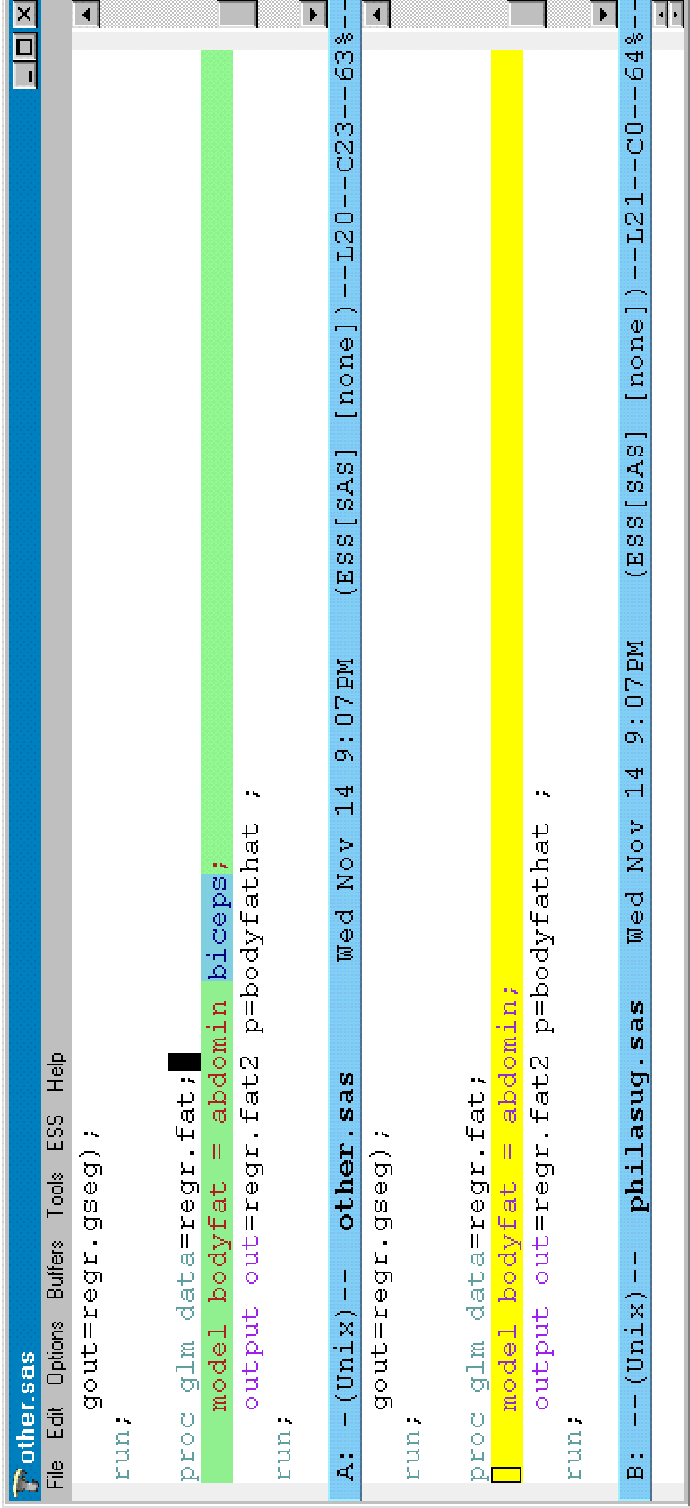
\includegraphics[angle=270,width=\textwidth]{ediff-sas}}
\url{http://www.analytics.washington.edu/downloads/ess/doc/figures/ediff-sas.gif}
  \caption{Ediff of two versions of a file.}
  \label{f.ediff}
\end{figure}

Comparison of files, two or three drafts of a paper for example, is
simplified by \stexttt{ediff}.  An example is shown in Figure
\ref{f.ediff}.  The lines that are similar are highlighted in the two
buffers, one for each file, and the specific words that mismatch are
highlighted in a contrasting color.  \stexttt{ediff} has many tools
for working with the differences in files and in entire directories.
When combined with the patch utility or a source-code control system,
it provides the user with the ability to insert, delete or modify only
the differing portions of text files.

% Rodney: You can't just mention complex functionality like etags and
% speedbar.  We would need to introduce these packages.  Since they
% aren't critical to ESS at this time, let's ignore them.
Emacs has many other important features.  Emacs provides file-manager
capabilities, such as \stexttt{dired} (discussed in Major and Minor
Modes above) and \stexttt{speedbar}, both of which interface to the
computer's directory structure.  Emacs stores the complete history of
commands issued in an editing session, allowing a flexible and fairly
complete undo capability.  More importantly, for modes which control
processes, the process input history is stored for recall as well as
for later editing for printing or re-use.  Emacs also includes web
browsers, mail/newsgroup readers, and spell checking.

In addition to being an extremely powerful editor, Emacs also
includes capabilities usually found in an operating system.  Thus, it
provides a strong foundation for constructing an integrated
development environment focused on the needs of statisticians.  Emacs'
power, flexibility, portability, and extensibility make it a solid
platform on which to construct a statistical analysis user interface.

\section{ESS extends Emacs}
\label{sec:ess-extends-emacs}

Statistical programming is the writing of computer programs for data
analysis and processing.  These programs might be written in a
computer language that requires a compiler, such as \Fortran\ or C.
But, more likely, they are written in a statistical analysis language
that only requires an interpreter such as R, \SAS, \Stata, or \XLispStat.
General purpose languages such as \Fortran, C/C++, Java, and PERL
have integrated development environments which facilitate writing and
debugging code.

ESS extends Emacs to provide an integrated development environment for
statistical languages.  It offers a single
interface for a variety of statistical computing tasks including
interactive data analysis and statistical programming.
ESS is able to provide a functional and extensible interface
which is uniform and consistent across multiple statistical packages.
This is done by adding shortcuts and features for accelerated editing
of files as well as by interacting with the particular statistical
packages to provide, for example, control of input/output, assistance
with evaluation, and specialized parsing of help files.

ESS supports the S family (S, \Splus, and R) interactively.  \SAS\ and
BUGS are also well supported for batch processing.  \Stata\ and
\XLispStat\ (including ARC and ViSta) are supported through
highlighting and process-interfacing.

\subsection{Features and capabilities}
\label{sec:ESS:features}

\paragraph{Syntactic highlighting and indentation of source code.}
The programmers task is eased when language constructs (such as
reserved words, function calls, strings, and comments) are visually
identifiable and when lines of code are automatically indented to a
depth appropriate to their context (e.g., if--then clauses, loops).
ESS provides both of these to the programmer by including a
description of the syntax of each supported statistical language in
the form used by \stexttt{font-lock-mode}.

Figure \ref{f.font} shows an example of font-locking a complicated S
statement.  The top panel shows an \stexttt{if} statement with a long
expression in the condition and a multi-line consequence.  The keyword
\stexttt{if} is shown in purple, the string \stexttt{"deltat"} in
RosyBrown.  The comments are in red.  Everything else is in the
standard font.  The consequence is indented and the continuations of
the consequence are further indented.  The matching parentheses are
shown in green.  The cursor is indicated by a solid box.  In the
bottom panel, we replaced the matching parenthesis with an unbalanced
bracket.  Emacs immediately marks that with the paren-mismatch font,
bright purple in this example.  On a black and white terminal we would
use bold, underline, italic, and reverse-video, rather than colors, to
distinguish the fonts.

% Figure \ref{f.font} shows a black-and-white example of font-locking a
% complicated S statement.  The top panel shows an \stexttt{if}
% statement with a long expression in the condition and a multi-line
% consequence.  The keyword \stexttt{if} is shown in an underlined font,
% the string \stexttt{"deltat"} in an italic underlined font.  The
% comments are in an italic font.  Everything else is in the standard
% font.  The consequence is indented and the continuations of the
% consequence are further indented.  The matching parentheses are marked
% by a bold foreground and a shaded background.  The cursor is indicated
% by a solid box.  In the bottom panel we replaced the matching
% parenthesis with an unbalanced bracket.  Emacs immediately marks that
% with the paren-mismatch font, bright purple on
% a color terminal.

The font selection and the indentation depth are automatically
supplied by Emacs as the lines are typed.  The user has several
options for mapping of colors or fonts to each of the syntactic types.
We selected
% black-and-white font-mapping for display here.  On a color terminal
% we might use
purple for the keywords, red for comments, green for matching parens,
and inverse-video purple for mismatched parens.  Emacs makes default
choices of colors and ESS provides several other optional schemes.

\begin{figure}[tbp]%h
%  \ESSfig{%
%    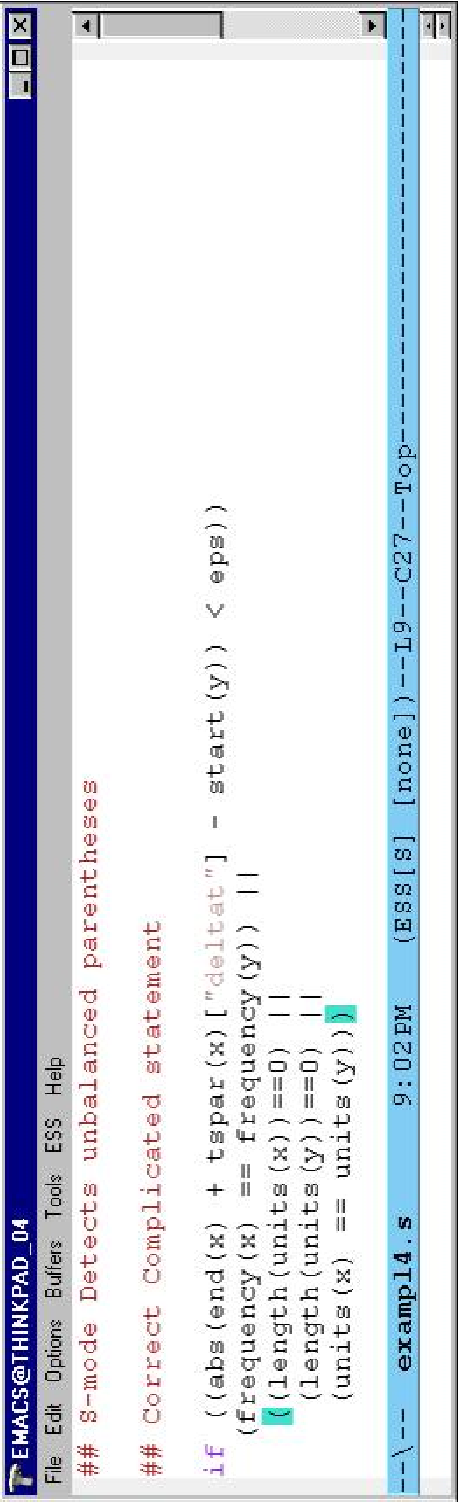
\includegraphics[angle=270,width=\textwidth]{font-cor-s}
%    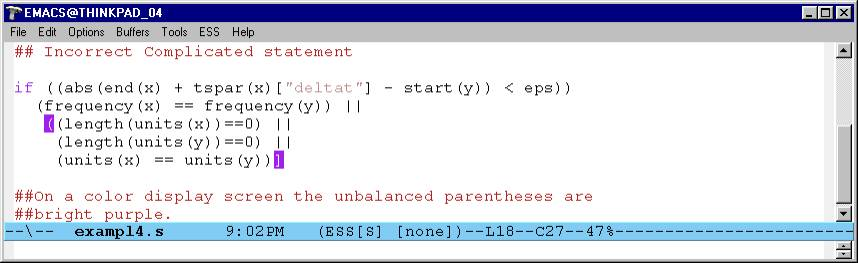
\includegraphics[angle=270,width=\textwidth]{font-incor-s}%
%    }
\url{http://www.analytics.washington.edu/downloads/ess/doc/figures/font-cor-s.jpg}
\url{http://www.analytics.washington.edu/downloads/ess/doc/figures/font-incor-s.jpg}
  \caption{We illustrate here with fonts and colors appropriate for a
    color display.  On a black and white terminal we would use bold,
    underline, italic, and reverse-video.  On a color terminal we
    would use a selection of colors.}
  \label{f.font}
\end{figure}

Since S syntax is similar to that of C, ESS uses the Emacs tools for
reformatting S code to match particular styles.  Common C format styles,
as well as locally customized styles, are defined by specifying the indentation
level for nested statements, location of open-braces (at the end or at the
beginning of a line), indentation offsets for if-then-else constructs,
and similar characteristics.

Syntax highlighting can be used to help enforce coding
standards.  Figure \ref{f.hilock} illustrates a standard for
\SAS\ programming that says all \stexttt{PROC} statements must use the
\stexttt{DATA=datasetname} option.

\begin{figure}[tbp]
%  \ESSfig{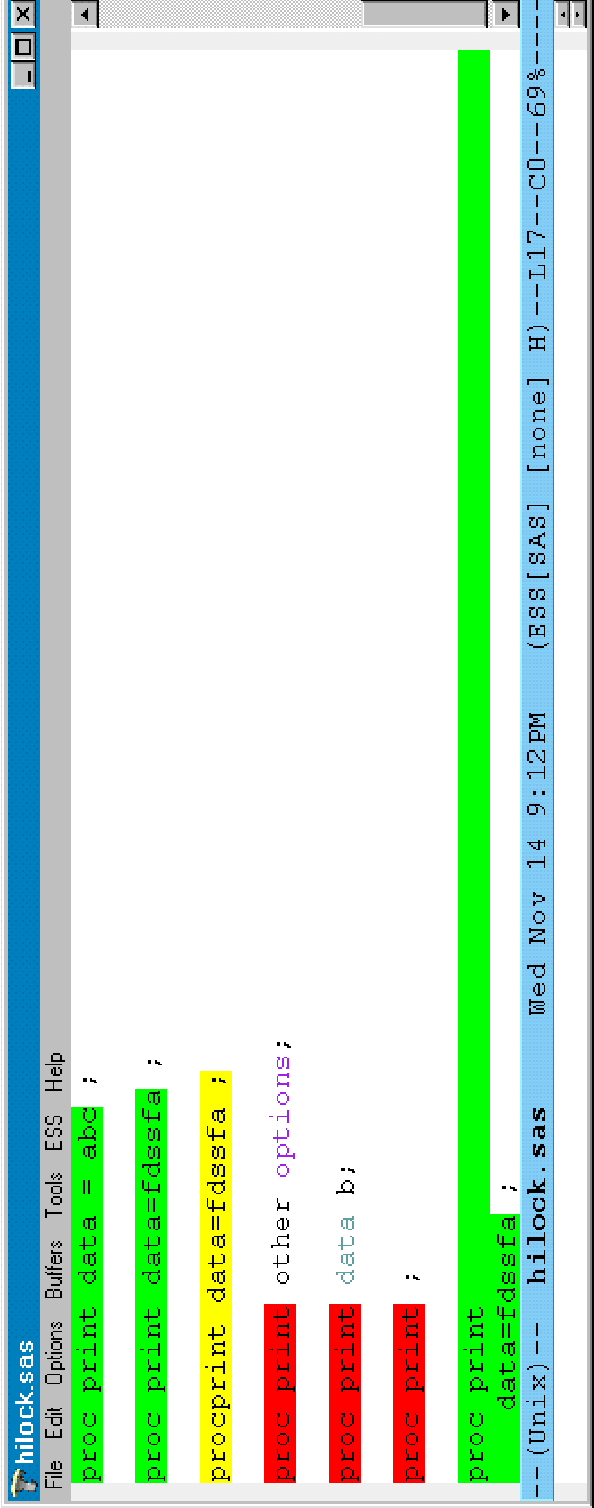
\includegraphics[angle=270,width=\textwidth]{hilock-sas}}
\url{http://www.analytics.washington.edu/downloads/ess/doc/figures/hilock-sas.gif}
  \caption{Enforce coding standards.  The standard here is
    that all \stexttt{PROC} statements must use the
    \stexttt{DATA=datasetname} option.  Lines that satisfy the
    standard turn green, lines that don't turn red.
    Ambiguous ones turn yellow.}
  \label{f.hilock}
\end{figure}

\paragraph{Process interaction.}
Emacs has historically referred to processes under its control as
``inferior'', accounting for the name inferior ESS (\stexttt{iESS}) to
denote the mode for interfacing with the statistical package.  Figure
\ref{f.ess-demo} shows the S language program \stexttt{ess-demo.s} in
the top buffer in \stexttt{ESS[S]} mode and the executing R process in
the bottom buffer \stexttt{*R*}.  The \stexttt{iESS} major mode of the
\stexttt{*R*} buffer is crafted for command-line editing.  This mode
remembers and uses the command history, allowing for the recall and
searching of previously entered commands.  Filename completion for
local directories is also available.

\begin{figure}[tb]
%  \ESSfig{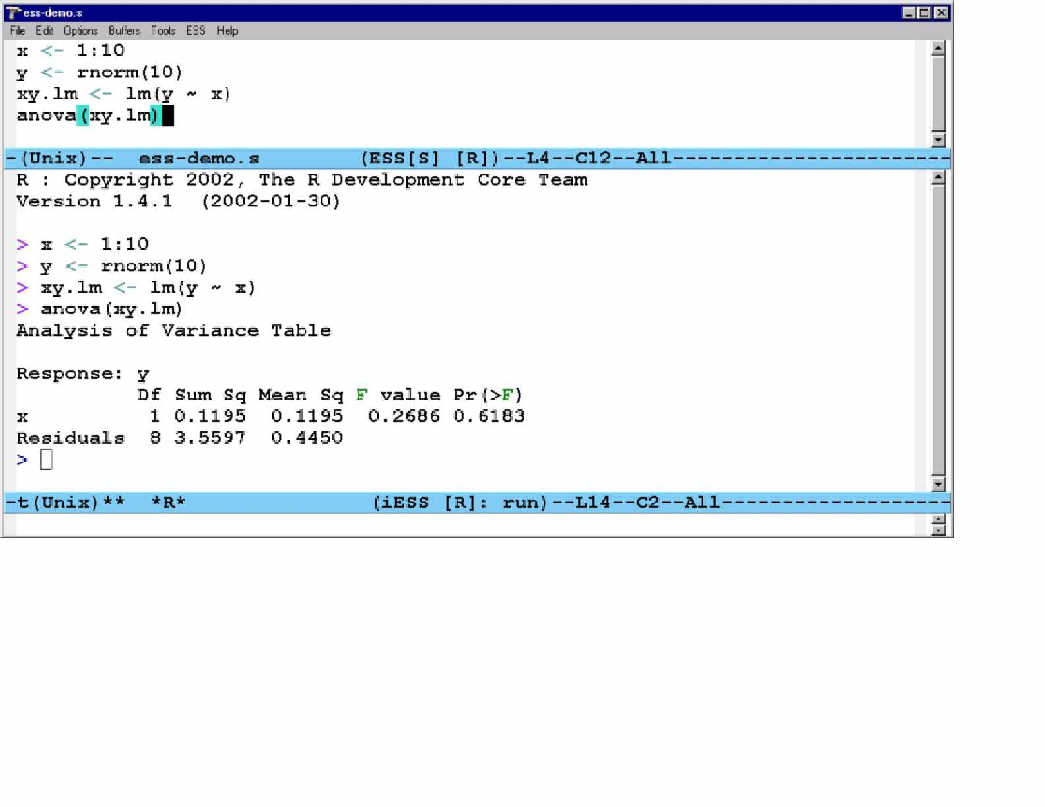
\includegraphics[angle=270,width=\textwidth]{ess-demo}}
\url{http://www.analytics.washington.edu/downloads/ess/doc/figures/ess-demo.jpg}
  \caption{Line-by-line execution of a command file. The cursor is
    placed on a line in the \stexttt{ESS[S]} buffer and then with a single
    key sequence
    the line is sent to the \stexttt{*R*} buffer for
    execution.  The output of the package goes directly to the
    editable \stexttt{*R*} buffer.}
  \label{f.ess-demo}
\end{figure}

\paragraph{Source-level Debugging.}
ESS facilitates the editing of source code files, sets of commands
written for a statistical analysis package, and allows the user to
load and error-check small sections of source code into the package.
This is done through several mechanisms.  First, the presence of
unbalanced parentheses or mismatched/unterminated quotes is
immediately evident with syntactic highlighting of the source code.
Second, functions are provided for simple and consistent execution of
user-specified or natural units of the code (function definitions in S
or \XLispStat, \stexttt{PROC \dots\ RUN;} sections in \SAS).  An
error-free evaluation lets the user execute the next section of code;
if errors arise, the user edits the current unit and re-evaluates.
Once the code is verified, an entire buffer, or file, of code can be
sent to the package as a unit.  This file can also be used as a batch
file for routine analysis at a later time.  Finally, output from the
statistics package is normally captured directly by Emacs and placed
into a buffer from where it can be edited and searched.  Particular
forms of output such as requests for help pages and log-file output
can be diverted into special buffers with modes crafted to facilitate
reading.  These modes include tools for automatically placing the
cursor on the first \stexttt{ERROR}, for example in \SAS\ and S.

\paragraph{Interactive transcripts.}
A transcript records all commands entered by the analyst and the
corresponding text-based responses such as tables and comments
generated by the statistics package during an interactive statistical
analysis session.  Once a transcript file is generated, for example by
saving an \stexttt{iESS} buffer, \stexttt{transcript-mode} assists
with reuse of part or all of the entered commands.  ESS understands
the transcript's syntax, especially the potential prompt patterns used
during the interactive analysis.  ESS provides tools to facilitate
editing and re-evaluating the commands directly from the saved
transcript.  This is useful both for demonstration of techniques and
for reconstruction and auditing of data analyses.  Special ESS
functions can ``clean'' S language transcripts by isolating all input
lines and placing them in a new S language source file.  Transcript
cleaning facilitates the use of an exploratory interactive analysis
session to construct functions and batch files for routine analysis of
similar data sets.

\paragraph{Remote access to statistics packages.}
ESS provides transparent facilities for editing files and running
programs which might reside on numerous remote machines during the
same session.  The remote machine could be a different platform than
the local machine.

\paragraph{Manipulating and Editing Objects (S family).}
For languages in the S family, ESS provides object-name completion of
both user- and system-defined functions and data.  ESS can dump and
save objects (user- and system-generated) into formatted text files,
and reload them (possibly after editing).

\paragraph{Help File Editing (R).}
ESS provides an R documentation mode (\stexttt{Rd-mode}) which assists
in writing help files for R functions, objects, and other topics worth
documenting.  \stexttt{Rd-mode} provides the ability to view and
execute code embedded in the help file in the same manner as ESS
handles code from any S language source file.  It provides syntax
highlighting and the ability to submit code directly to a running ESS
process, either R or \Splus, for evaluation and debugging.  This
latter feature is useful for ensuring that code developed using R runs
under \Splus.

\paragraph{Cooperation across Multiple Tools.}
Statistical packages are intended for either general statistical
analyses or for specialized forms of statistical analyses.  The
specialized statistical packages can be far more efficient for their
intended activities, but this is balanced by their inability to
perform a wide range of general statistical functions.  Tightly
coupled inter-operability between general and specialized packages
rarely exists, but such a facility is often desired.  For example, a
general purpose package such as R does not perform Bayesian analyses
as easily as BUGS does.  On the other hand, BUGS lacks breadth in the
range of analyses and results it can generate.  For this reason, BUGS
is often distributed with R packages, like the diagnostic packages
CODA and BOA, which assist with importing and analyzing the results in
R.  Another point of contention is the difference in the interfaces
between general packages and specialized packages.  ESS helps by
providing a single point of contact to both tools, though the typical
interfaces (interactive for R, batch for BUGS) are different.

%\item[Rodney:]  I can't speak for everyone, but the BUGS users I know are
% .. lots deleted by AJR
%will make sense.  Besides, the most pressing need for me is to get
%ESS-elsewhere to work with ESS[BUGS] rather than creating inferior-BUGS.

%\item[Rich:] How does making ``ESS-elsewhere work with ESS[BUGS]'' differ
%from ``creating inferior-BUGS''?  My question is predicated on the assumption
%that ESS-elsewhere is a (generalized) minor-mode that makes the location
%of the program irrelevant.
%See my ESS-elsewhere quibble below.

%\item[Rodney:] It's the whole batch BUGS vs. interactive BUGS thing.  Batch
%BUGS with ESS-elsewhere; interactive BUGS with inferior-BUGS which does not
%and will never exist.  If you want to call ``inferior-ESS'' ``ESS-elsewhere''
%why do you need two different names?  ``inferior-ESS'' is a terrible name
%so the change would be fine with me, but you can't have it both ways?  Is
%this why you keep saying that ESS-elsewhere works for SAS?  See
%response to quibble below.

%\item[Rich:]
%\stexttt{iESS[SAS]} was designed to mimic as well as possible \stexttt{iESS[S]}.
%I need to read doc/README.SAS to make sure all of its options are represented
%here. --- Not yet done.
%\end{description}
%\end{Comment}

\paragraph{Simplifying Keymap Differences.}
Simple conflicts between interfaces are exemplified by different key
sequences for editing tasks such as cut, copy, paste, beginning of
line, end of line, etc.  These may be the most aggravating because our
fingers are typing ``instinctively'', but differences in interfaces
circumvent this learned behavior.  ESS solves this problem by
providing a uniform interface to keyboard actions across the variety
of statistical packages that might be used.  That is, the same key
sequences are used for cursor movement, evaluation, and basic tasks
such as loading files for editing.

\paragraph{Concurrent Use of Multiple Machines and Operating Systems.}
It can be useful to have multiple statistical processes running
simultaneously, either on a single machine or a variety of machines.
This capability assists with large-scale numerical simulations as well
as code design and testing across multiple versions of statistical
software packages.

\subsection{Interactive Processing.}
\label{sec:interactive}

The increased popularity of exploratory data analysis as well as the
advent of simple GUIs has made interactive data analysis an important
component to statistical practices.
ESS uses three different approaches for communicating with statistical
packages.

\paragraph{Inter-Process Communication.}
Packages that use the command-line interface are run as an inferior
process in an Emacs buffer, with the standard input and output of the
package redirected to the buffer.  Packages that do not use the
command-line interface must be run as an independent process, possibly
with limited cooperation.

ESS can use the Windows DDE (Dynamic Data Exchange) protocol to
provide one-way communication directly to packages which function as a
DDE server.  ESS can control the actions of the package, but it can not capture
the results directly.  Transcripts must be physically copied to an
Emacs buffer to get the transcript editing features.

Statistical packages that use neither the standard input/standard
output protocol nor DDE can not be directly controlled by Emacs.  But, ESS
can still provide an editing environment for these statistical languages.  The
user must either manually cut and paste the edited code into the
package or save the edited files and run them in a batch environment.
The Microsoft Windows versions of \SAS, \Stata, and \XLispStat\ are
in this category.

One useful extension in ESS is relaxation of the requirement that the
statistics program be available on the local machine.  ESS provides
both transparent editing of files and execution of statistics packages
on a remote machine with \stexttt{iESS[S]} or \stexttt{iESS[SAS]} (see
below).  All the editing and interaction features described for the
local machine work equally well on the remote machine.  The
interaction, including all the unique features of working with ESS,
appears to the user as if the program were running on the local
%rmh: The interaction ... appears ....
machine.  If the X11 Windowing system is running on the local machine,
it is even possible to bring up visual displays and graphics from
remote Unix systems onto a local Microsoft Windows or Apple Mac
display.

\paragraph{Interactive S family}
ESS for S family statistical languages, \stexttt{iESS[S]},
replaces the \Splus\ Commands window or the R GUI window.  In addition
to running the S family language process, \stexttt{iESS[S]} mode provides the
same editing features, including syntactic highlighting and
string-search, as the editing mode \stexttt{ESS[S]}.  It also provides
an interactive history mechanism; transcript recording and editing;
and the ability to re-submit the contents of a multi-line command to
the executing process with a single keystroke.  \stexttt{iESS[S]} is
used with S, \Splus, and R on Unix and with Sqpe and R on Windows.

The \Splus\ GUI on Windows can be a DDE server.  There are two
advantages to using even this limited communication with the \Splus\
GUI through ESS.  First, through \stexttt{ESS[S]} mode the user gets
the full editing capabilities of Emacs.  Second, S language commands
% rmh: S, not \Splus, in both places.  The {\it language} is S.
% The previous session could be R or ATT S.  It is not restricted to \Splus.
are sent from the editing mode \stexttt{ESS[S]} buffer and from
transcript buffers from previous S sessions directly to the GUI
Commands window with the same Emacs key sequences as are used with ESS
on Unix.  Hence the user can work in a powerful editing environment
and is protected from the delay and ergonomic challenges of using the
mouse for copy and paste operations across windows.

\paragraph{Interactive \SAS.}
\stexttt{iESS[SAS]} is a mode that allows text-based \stexttt{PROC} by
\stexttt{PROC} interaction with an inferior buffer running an
interactive \SAS\ session on either the local or a remote computer.
\stexttt{iESS[SAS]} mode works by redirecting standard input and
output from \SAS\ to ESS.  Currently, the \stexttt{iESS[SAS]} mode can
run on any computer, but the \SAS\ process it is controlling must be
running on a Unix machine.  This process is very efficient for dial-up
network connections to a remote computer with \SAS\ installed.  The
resulting interface is similar to the SAS character terminal
interface, but with Emacs key sequences.

%Rodney:  What is this paragraph about?  I'm going to comment it out
%because I don't recognize what it is supposed to be.  Maybe somebody
%can fix it later.
%
% rmh: Round umpteen.  Yes, this is redundant with the third paragraph
% of interprocess communication.  I still want it here.  Try this rephrasing.
%
\stexttt{ESS[SAS]} mode can be used in conjunction with the \SAS\
Display Manager to allow simultaneous access to Emacs for editing
\SAS\ language code and to the \SAS\ mouse-based interfaces to the
graphical routines and help system.

%%%%% AJR: WHY IS THIS SUBSTANTIALLY DIFFERENT THAN BATCH?  I KNOW ITS
%%%%% SLIGHTLY DIFFERENT, BUT SUBSTANTIALLY?
%%%%% rmh: this is a form of interaction, not batch.  I restored the
%%%%% first paragraph with some expansion.
%\paragraph{\SAS---Interactive cooperation with the \SAS\ Display Manager.}
%ESS users who write data analysis code in \stexttt{ESS[SAS]} mode in Emacs
%often need to work with the \SAS\ Display Manager's
%mouse-based interface to the graphical
%routines, the help system, and other non-text-based features.
%%The authors of ESS prefer the Emacs environment for
%%the text-file interaction with \SAS, that is with editing and
%%managing input command files and output listing and log files,
%%even on computer systems which run
%%the \SAS\ Display Manager environment.
%In this situation, the user
%designs the command file in \stexttt{ESS[SAS]} mode and highlights
%regions to be forwarded to \SAS\ for processing.
%%
%% Rodney: I don't see this as a feature of either ESS or emacs.  And,
%% what the authors prefer is certainly not germane.
%%
%%
%% rmh: This is my preferred mode for interacting with SAS.  I tried another
%% rephrasing.  It {\it is} a feature of ESS.  ESS is able to provide ESS[SAS]
%% mode for the text processing (.sas .lst. log files) and simultaneously
%% let the user have interactive graphical access.
%%This can be done by either:
%%\begin{enumerate}
%%\item copying and pasting the marked regions to the \SAS\ Editor window
%%  and then pressing the \stexttt{RUN} button.  Highlighted sections of
%%  the \SAS\ Listing window are brought back to Emacs to be read in the
%%  \stexttt{ESSlst} mode editing environment.
%%\item submitting the marked region for Batch File Processing (see the
%%  next section) but using the mapped key sequences to append to the log
%%  and listing files instead of replacing them.
%%\end{enumerate}

\subsection{Batch File Processing.}
\label{sec:batch-file}

Batch file processing with statistical analysis packages is a better
choice than interactive processing when the execution times are longer
than the user is willing to wait as well as for regularly updated
statistical reports and figures.  ESS provides a means to shorten the
debugging cycle for writing code intended for batch evaluation by
containing the whole process, both writing and evaluation, within
Emacs.

\paragraph{Batch \SAS.}
\label{sec:sas-batch}

\SAS\ is a popular choice for processing and analyzing large amounts
of data.  However, interactive \SAS\ is rarely used in these situations
due to the length of time involved.  Instead, a file containing \SAS\
commands is created and \SAS\ executes these commands in the background,
or batch, while the user moves on to other activities.

ESS facilitates \SAS\ batch with \stexttt{ESS[SAS]}, the mode for files
with the \stexttt{sas} extension.  ESS defines \SAS\ syntax so that
\stexttt{font-lock-mode} can highlight statements, procedures,
functions, macros, datasets, comments and character string literals in
\SAS\ programs.  Optionally, the same language features are
highlighted in the \SAS\ log with the addition of log notes, warnings
and error messages.

For files with the \stexttt{sas} extension, ESS binds the function
keys in \stexttt{ESS[SAS]} mode to match the definitions used by \SAS\
Display Manager.  These definitions are optionally available in all
modes.  They are particularly useful when viewing \SAS\ log and
listing files (with extensions of \stexttt{log} and \stexttt{lst}
respectively).

Only one function key press is needed to submit a \SAS\ batch process.
Other function keys open the \SAS\ program, the \SAS\ log and the
\SAS\ listing buffers.  When accessed in this manner, the \SAS\ log
and \SAS\ listing buffers are automatically updated since they may
have been appended or over-written by the \SAS\ batch process.  In
addition, the \SAS\ log is searched for error messages and the error
messages, if any, are sequentially displayed with consecutive key
presses.

Another function key opens a \SAS\ permanent dataset for editing or
viewing.  An option is provided so that the tab and return keys
operate in typewriter fashion like they do in \SAS\ Display Manager.
This option also defines a key to move the cursor to a previous
tab-stop and delete any characters between its present position and
the tab-stop.  This is a \SAS\ Display Manager feature that is not
typically available in Emacs.

The \SAS\ batch process runs on the computer where the \SAS\ program
resides.  This is important because any \SAS\ permanent datasets
referenced in a \SAS\ program only exist on the computer running \SAS.
If the \SAS\ program resides on a remote computer, then the
log and listing are also accessed remotely.  The net result is that
running \SAS\ batch on remote computers is nearly transparent to the
ESS user.

%\begin{Comment}
%Rich's version:
%\end{Comment}
%The \SAS\ batch process can run on the same computer on which the
%emacs session is running or it can run on a remote computer.  For
%remote jobs, files are transparently saved (with ftp or scp or kermit)
%and the batch process is transparently submitted through a telnet or
%ssh connection.

%\begin{Comment}
%Rich: I have some terminology quibbles here with how the term
%``ESS-elsewhere'' is used with SAS BATCH.  I think of S-elsewhere or
%ESS-elsewhere as a trick to make a \stexttt{telnet-mode} buffer think
%it is \stexttt{iESS-mode} buffer.

%I don't think of file saving, editing, and retrieval as an example
%of ESS-elsewhere.   Neither is submission of the remote job;
%that is just an ordinary shell command in an ordinary shell buffer.
%M-x SAS probably is an example of ESS-elsewhere, but I
%designed it before I thought of the ESS-elsewhere concept.

%The initial idea behind S-elsewhere was to run an interactive S or S-Plus
%session on a remote computer in telnet (or equivalent) buffer.  The trick
%was to make the \stexttt{telnet-mode} buffer accept C-c C-n and
%related commands from the \stexttt{S-mode} buffers.  Hence I had to
%make the \stexttt{telnet-mode} buffer think it is \stexttt{iESS-mode}
%buffer.  The ``elsewhere'' part of the name is entirely related to a
%different start up procedure.  Once the connection is made, there is
%{\em no} difference visible to the user.  The buffer shows itself to
%be an ordinary \stexttt{iESS} buffer.  Tony generalized S-elsewhere
%to ESS-elsewhere to allow other languages than S to be used
%interactively.

%I have been using ESS for SAS remote BATCH for years, ever since you
%and I started working on this together.  We initially defined
%ess-sas-submit-method to encapsulate the location of the sas process.
%Except for a few lines of elisp to get the connection started, the user
%behavior has been identical whether the SAS process is on the same or
%different machine.  Since we are not interactively talking to the SAS
%process in an inferior-ESS buffer I don't see this as ESS-elsewhere.

%Rodney: Remote submissions of SAS batch jobs never worked.  I only got
%it to work a couple of weeks ago.  The problem was with the cd command.
%You need to ignore the beginning and end of the expanded buffer name
%that are the ange-ftp/EFS/tramp stubs which tell Emacs what the remote
%username and hostname are.  I find the batch usage of ESS-elsewhere
%entirely consistent with the interactive behavior.  OTOH, I don't find
%the terminology particularly illuminating.  I think ESS-remote or
%ESS-net would be more meaningful.
%\end{Comment}

\paragraph{Batch BUGS.}
BUGS software performs Markov Chain Monte Carlo integration.  There is
an interactive capability, but it is not often used since the analyses
can be very time-consuming.  Most BUGS programs are executed as batch
processes.  ESS facilitates BUGS batch with \stexttt{ESS[BUGS]}, the
mode for files with the \stexttt{bug} extension.  ESS provides 4
features.  First, BUGS syntax is described to allow for proper
fontification of statements, distributions, functions, commands and
comments in BUGS model files, command files and log files.  Second,
ESS creates templates for the command file from the model file so that
a BUGS batch process can be defined by a single file.  Third, ESS
provides a BUGS batch script that allows ESS to set BUGS batch
parameters.  Finally, key sequences are defined to create a command
file and submit a BUGS batch process.

\paragraph{Batch S family.}
ESS provides 2 facilities for batch processing of S family language files.
The first is to execute the contents of a file using buffer-evaluation.  This
differs from interactive processing only by the number of commands
being evaluated; errors can be found by examining the resulting
transcript.  The second is the load-source mechanism, which provides a
means of jumping to errors in the source file, but doesn't display the
evaluated commands in the transcript.  These mechanisms provide
different tools for debugging the source files.

\section{History of ESS}
\label{sec:ESS:history}

ESS is built on Emacs, the editing system for which Richard Stallman
won a MacArthur Foundation Fellowship in 1990.  Emacs has a long
history of being a programmer's editor.  Many statisticians got their
first taste of the power of Emacs with \Fortran\ mode which was
introduced in 1986.  As statisticians' preferences changed from
generalist compiled languages such as \Fortran\ to specialist
statistical analysis packages like S and \SAS, Emacs modes soon
followed.

The ESS environment is built on the open-source projects of
many contributors, dating back over 10 years.
Doug Bates and Ed Kademan wrote S-mode in 1989 to edit S and \Splus\
files in GNU Emacs.  Frank Ritter and Mike Meyer added features,
creating version 2.  Meyer and David Smith made further contributions,
creating version 3.  For version 4, David Smith provided significant
enhancements to allow for powerful process interaction.

John Sall wrote GNU Emacs macros for \SAS\ source code around 1990.
Tom Cook added functions to submit jobs, review listing and log files,
and produce basic views of a dataset, thus creating a SAS-mode which was
distributed in 1994.

In 1994, A.J. Rossini extended S-mode to support XEmacs.  Together
with extensions written by Martin M{\"a}chler, this became version
4.7 and supported S, \Splus, and R.
In 1995, Rossini extended SAS-mode to work with XEmacs.

In 1997, Rossini merged S-mode and SAS-mode into a single Emacs
package for statistical programming; the product of this marriage was
called ESS version 5.  Richard M. Heiberger designed the inferior mode
for interactive \SAS\ and SAS-mode was further integrated into ESS.
Thomas Lumley's Stata mode, written around 1996, was also folded into
ESS.  More changes were made to support additional statistical
languages, particularly \XLispStat.

ESS initially worked only with Unix statistics packages that used
standard-input and standard-output for both the command-line interface
and batch processing.  ESS could not communicate with statistical
packages that did not use this protocol.  This changed in 1998 when
Brian Ripley demonstrated use of the Windows Dynamic Data Exchange
(DDE) protocol with ESS.  Heiberger then used DDE to provide
interactive interfaces for Windows versions of \Splus.  In 1999,
Rodney A. Sparapani and Heiberger implemented \SAS\ batch for ESS, which
relies on files rather than standard-input/standard-output, on Unix,
Windows and Mac.  In 2001, Sparapani added BUGS batch file processing
to ESS for Unix and Windows.

This history is summarized in Table \ref{tab:timeline}.

\begin{table}[tbp]
  \centering
  {\scriptsize
  \begin{tabular}{c ll c ll}
\hline
    Year  \\
\hline
         & \multicolumn{2}{c}{S-mode}       && \multicolumn{2}{c}{SAS-mode} \\
\cline{2-3} \cline{5-6}
    1989 & v.1 & (GNU Emacs, Unix, S/S+)        &&  \\
    1990 &     &                            &&     & (GNU Emacs, Unix, SAS editing) \\
    1991 & v.2 & (GNU Emacs, Unix, S/S+)        && \\
    1993 & v.3 & (GNU Emacs, Unix, S/S+)        && \\
    1994 & v.4 & (GNU Emacs/XEmacs, Unix, S/S+) && v.1  & (GNU Emacs, Unix, SAS batch) \\
    1995 & v.4.7 & (GNU Emacs/XEmacs, Unix, S/S+/R) && v.2 & (GNU Emacs/XEmacs, Unix, SAS batch) \\
    \cline{2-6}\\[-3.5ex]
    \cline{2-6}
         & \multicolumn{5}{c}{Emacs Speaks Statistics (ESS)} \\
    \cline{2-6}
         &\multicolumn{2}{c}{Emacs, Operating Systems} &&\multicolumn{2}{c}{Additional Functionality}\\
\cline{2-3} \cline{5-6}
    1997 & v.5.0 & (GNU Emacs/XEmacs, Unix)         &&&  Stata, XLispStat, SAS interactive \\
    1998 & v.5.1.1 & (GNU Emacs/XEmacs, Unix/Windows) &&&  S+elsewhere; Windows: S+/R\\
    1999 & v.5.1.10 & (GNU Emacs/XEmacs, Unix/Windows/Mac) &&& SAS batch; Omegahat \\
    2001 & v.5.1.19 & (GNU Emacs/XEmacs, Unix/Windows/Mac) &&& Unix/DOS: BUGS batch; Mac: R \\
%%    2002 & v.5.1.20 & (Emacs/XEmacs, Unix/Windows/Mac) &&& Unix/DOS: BUGS batch, Mac: R \\
%%    2002 & v.5.2 & (Emacs/XEmacs, Unix/Windows/Mac) &&& ? \\
    \hline
  \end{tabular}
  }
  \caption{History and Ancestors of ESS}
  \label{tab:timeline}
\end{table}


%\section{Future Work}

%%%There are two active areas of extensions for user environments.  One
%%%is to enhance the capabilities of the IDE for statistical practice;
%%%this includes implementing such common IDE features as object
%%%browsers, tool-tips, and interfacing cleaning.  The other is to target
%%%appropriate potentially useful programming methodologies for transfer
%%%to statistical practice.
%%%
%%%Literate Programming methodologies \citep{Knuth:1992,NRamsey:1994} are
%%%a natural fit for statistical practice.  We refer to the application
%%%to statistical analysis as Literate Statistical Practice
%%%\citep{rossini:dsc:2001}.  The tools used are Noweb
%%%\citep{NRamsey:1994} and either \LaTeX, \textsc{html}, or \textsc{xml}
%%%for documenting and explaining the analysis.  This approach to
%%%programming encourages the use of a literary documentation style to
%%%explain the programming code for the data analysis.  The program can
%%%then be extracted from the documentation text for realizing the
%%%statistical analysis.

%%future enhancement perhaps
%%ESS provides the same ESS-elsewhere support for BUGS batch
%%that it does for \SAS\ batch (see above).

%Important extensions which should be implemented in future
%versions include class browsers, analysis templates, tool-tips, and
%similar features.  Class browsers can be thought of as a tree or
%outline for presenting datasets, variables and functions in the
%context of what they represent; this allows for rapid and appropriate
%inspection.  Analysis templates would allow statistics centers and
%groups to provide standardized templates for initiating an analysis.

%Additional statistical packages can easily be added to ESS.

%%While most IDE features have been developed for object-oriented
%%languages, the above also can apply to non-object oriented
%%programming.

%ESS is one of the first  Rapid Application Development (RAD)
%environments intended for statisticians.  It provides


\section{Conclusion}
\label{sec:concl}

ESS provides an enhanced, powerful interface for efficient interactive
data analysis and statistical programming.  It allows the user
complete control over the communications among the files in which the
analysis is specified, the statistical process doing the computation,
and the output.  Because all are within the same programming
environment, and therefore are accessed with the same editing and
searching concepts and the same key sequences, user efficiency is
increased.  It is completely customizable to satisfy individual
desires for interface styles and can be extended to support other
statistical languages and data analysis packages.

%\begin{Comment}
%Rich: see my discussion of ESS-elsewhere terminology.

%What is the behavior for remote SAS that is new for 2002?

%Rodney: SAS batch now works and Kermit was added as a method of transfer.
%\end{Comment}
%ESS-elsewhere provides interactive and batch processing
%with \SAS\ running on a remote machine that is accessed over a
%network.  This provides a powerful development environment for \SAS.

%%This
%%includes support for syntax highlighting and template-based source file
%%generation that provides the capability of specifying all the necessary
%%parameters for a BUGS batch run in a single file.

\bibliographystyle{plainnat}
\pdfbookmark[1]{References}{section.7}
%\addcontentsline {toc}{section}{\numberline {}References}
\bibliography{ess-intro-graphs}

\clearpage

\appendix
\section{Appendix: ESS Resources on the Internet}
%\addcontentsline {toc}{section}{\numberline {}ESS Resources on the Internet}
\label{sec:access}

\paragraph{Latest Version.}

ESS is constantly in flux.  New versions of statistical
packages, Emacs and operating systems require new releases of ESS to
support them.  The latest stable version of ESS can be found on the web at
\url{http://www.analytics.washington.edu/downloads/ess/}.  To get help
with problems, send e-mail to \url{mailto: ess-help@stat.math.ethz.ch}.
The latest development, hence unstable, version can be obtained by
anonymous CVS.  First type:

\stexttt{cvs -d
  :pserver:anoncvs@cvs.analytics.washington.edu:/var/anoncvs login}

You will be prompted for a password which is ``\stexttt{anoncvs}''.
Then type:

\stexttt{cvs -d
  :pserver:anoncvs@cvs.analytics.washington.edu:/var/anoncvs co
  ess}

\paragraph{Additional documentation.}

An expanded version of the present paper is in \citep{RMHHS:2001}.  A
general introduction and usage instructions can be found in
\citep{heiberger:dsc:2001}; in addition, one which is more focused on
\SAS\ can be found in \citep{heiberger:philasugi:2001}.  The
documentation that comes with ESS provides details of its
implementation as well as examples of its use.

\end{document}


%%% Local Variables:
%%% mode: latex
%%% TeX-master: t
%%% End:
